\section{Chapter Overview}
This chapter explains the core implementation of the research prototype together with the technologies, languages \& supporting tools used for development of the prototype, with reasoning to the choice of each selection.

\section{Technology Selection}

\subsection{Technology Stack}
The technologies that were used to implement the prototype at each layer are shown below.
% Technologies used in various tiers or layers using a diagram.

% canva design: https://www.canva.com/design/DAEr30kH33k/mLBvcR5DptGOwK55cJddvA/edit

\begin{figure}[h!]
\centering
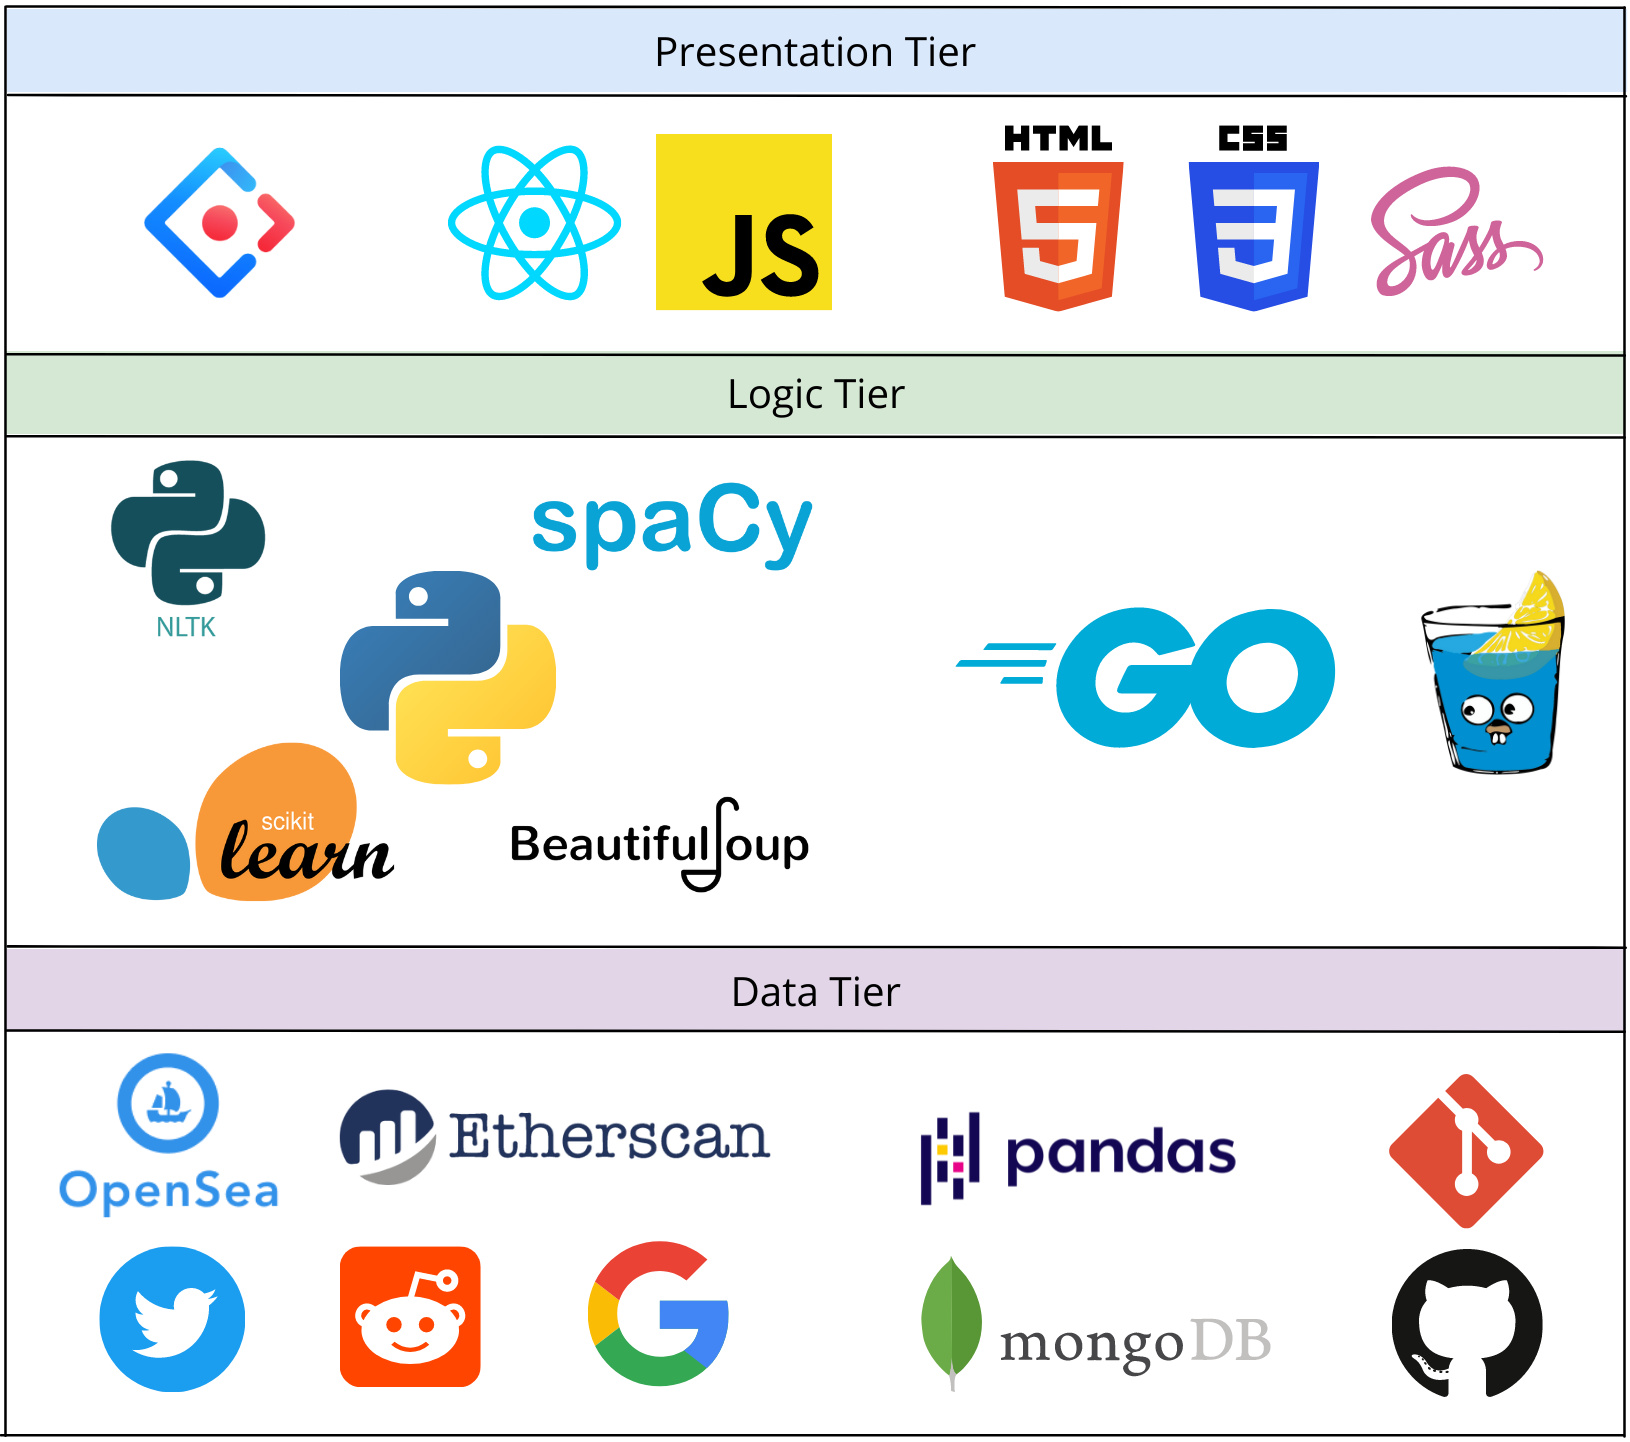
\includegraphics[width=0.8\textwidth]{images/Implementation/tech-stack.png}
\caption{Technology Stack}
\label{fig:teck-stack}
\end{figure}

% TODO: add a description (if not described later)
% \blindtext



\subsection{Data Selection}
% Data Selection (if data science project)
Being a data science project at the core, it was important to choose the best possible sources of data to gather sufficient data for analysis \& produce the best possible recommendations.

The data requirements identified were,
\begin{enumerate}
\item \gls{nft} asset data
\item Global trends data
\item \gls{nft} Smart Contract data
\item \gls{nft} events (sales) data
\item \gls{nft} bids data
\end{enumerate}

Since the main technological research gap to be addressed was with the integration of global trends into content based recommendations, this was given a higher priority at first.
These data requirements were sourced from the following sources and heavily pre-processed there after to create a usable dataset for data analysis. 

\begin{itemize}
\item \gls{nft} asset, events, bids data - From the \textbf{OpenSea API}.
\item Global trends data
\begin{itemize}
    \item Twitter data - From \textbf{Twitter developer API}.
    \item Google Trends data - From Google Dataset Search \& unofficial \textbf{Google Trends Python API (Pytrends)}.
%     \item Reddit data - From the Reddit API.
\end{itemize}
\item Ethereum Smart Contract data - From Etherscan \& OpenSea
% \item \textbf{User Preference Profiles data} - From Amazon, Yelp, Kaggle open datasets. May be needed for testing purposes.
\end{itemize}


All the data-points that could be used for recommendations and explored with iterative development, as a research. This iterative process took a long time since the \gls{api}s were rate limited. The gathered pre-processed datasets will be made available for public use for future researches.

\subsection{Selection of development framework}
% Use a table to justify your selection for each of them.
\vspace{-4mm}
\begin{longtable}{|p{0.16\linewidth}|p{0.8\linewidth}|}
\caption{Selection of development framework}\\ 
\hline
\textbf{Framework} & \textbf{Justification for selection}\endfirsthead 
\hline
Gin Gonic & It's extremely convenient to build \gls{api}s using Gin with Golang. It also has an easily debuggable log output \& claims smashing performance (up to 40 times faster!)\\
\hline
Ant Design & The world's second most popular React UI framework. Used in many industrial applications and has a wide range of components to match most UI requirements. Since it's tree-shaking compatible, it will build only the components that are used. This reduces build time of the frontend. The CSS is easily customizable as well. \\ 
\hline
\end{longtable}

Although this is a data science project, all data science models utilized were built from scratch without the use of libraries, since doing so allowed the author to tweak the models at will.

% -----

\subsection{Programming language}
% Justify what you’re using, why you’re using it.
\textbf{Python} is the language that will be used to create the \gls{ml} models.  Python is an all-purpose language that has been used in many projects involving data science. It has a vast collection of supporting libraries that eases many data science related tasks.

For the \gls{api} proxy it was decided to use \textbf{Golang}, which is statically typed language that attempts to resemble the performance of C. Golang will allow the application to support concurrency and multi-threaded communications while being extremely lightweight and fast. This will be used to avoid any bottlenecks that could occur at this point in the system, while potentially bolstering performance.

For the frontend, \textbf{JavaScript} was decided to be used to show dynamic content and allow a highly interactible \& inviting user experience.

\subsection{Libraries Utilized}
% Tabular form and justify.
\vspace{-4mm}
\begin{longtable}{|p{0.16\linewidth}|p{0.8\linewidth}|}
\caption{Libraries Utilized with justification for choices}\\ 
\hline
\textbf{Library} & \textbf{Justification for selection}\endfirsthead 
\hline
% data science python libraries used
Pandas & Pandas dataframes allow a vast range of functionalities required for data analysis such as cleaning, transforming, filtering, sorting \& manipulating of data \\
\hline
Scikit-learn & Used for vectorizing text and generate similarity matrices between items, for recommendations. \\
\hline
NLTK & Convenient to use for \gls{nlp} data parsing, using the RAKE vectorizer. \\
\hline
SpaCy & Allows production-ready advanced \gls{nlp}. \\
\hline
Beautiful Soup & Convenient to scrape data from the internet. \\
\hline
Matplotlib & Has almost any type of visualization method for data analysis. \\
\hline
React & A UI library that makes it easy to build interactive websites. Used as an alternative to using a framework since the vast array of capabilities and other integratable frameworks and libraries. It was important to develop an easily interactible frontend, since it will be the users’ point of interaction with the system. \\
\hline
\end{longtable}

\subsection{IDE’s Utilized}
% Tabular form and justify.
\vspace{-4mm}
\begin{longtable}{|p{0.16\linewidth}|p{0.8\linewidth}|}
\caption{IDEs Utilized with justification for choices}\\ 
\hline
\textbf{IDE} & \textbf{Justification for selection}\endfirsthead 
\hline
Google Colab & Convenience of trial \& error of fetching data, building, testing \gls{ml} models and ability to work across multiple devices with the cloud development environment. \\
\hline
VSCode & Extremely dynamic while being simple to use, yet powerful for front-end development with it's extensions \& code snippets. \\
\hline
Golang & Convenient syntax highlighting \& auto-completion for Golang development. \\
\hline
PyCharm & Well-equipped Python \gls{ide} with a lot of capabilities.\\
\hline
\end{longtable}


\subsection{Summary of Technology selection}
% tabular form
\vspace{-4mm}
\begin{longtable}{|p{0.3\linewidth}|p{0.65\linewidth}|}
\caption{Summary of Technology selection}\\ 
\hline
\textbf{Component} & \textbf{Tools}\endfirsthead 
\hline
Programming Languages & Python, Golang, JavaScript \\
\hline
Development Framework & Gin Gonic \\
\hline
UI Framework & Ant Design of React \\
\hline
Libraries & Pandas, Scikit-learn, NLTK, SpaCy, Beautiful Soup, Matplotlib, React \\
\hline
IDE – Research & Google Colab \\
\hline
IDE – Product & VSCode, Golang, Pycharm \\
\hline
Version Control & Git, GitHub \\
\hline
Application hosting & Netlify, AWS,
% Google Cloud App Engine?
\\
\hline
\end{longtable}


\section{Implementation of core functionalities}
% Discuss core functionalities with support of code segments.

% Since a Recommendations System's ultimate goal is to reduce the amount of information overload and

% nft data extraction

% nlp pre processing

% vectorizing

% matching

% ensembling

\section{Self-Reflection}
% reflection on your current prototype.

% Results of evaluation metrics and if possible also have the qualitative evaluation - check across a time period, how the recommendations vary and appear to be timely compared to recommendations produced without integrating social trends.

\section{Video Demo}
% Upload video to Youtube as unlisted video and provide Link to video demo
The link to the demo video presenting the current implementation progress can be found here: \url{https://www.youtube.com}

\section{Chapter Summary}
The chapter comprised of the technologies, languages \& supporting tools utilized to implement the prototype developed as part of the research. Discussions accompany the code snippets and algorithms produced as part of core functionality. Finally, the author's self-reflection of the developed prototype was presented.
